
在已經瞭解過的順序數據結構中,數據都存儲在一個數組中(或者是一個由內存塊組成的數組)。現在將考慮一種不同類型的數據結構,其中數據是通過指針連接在一起的。最簡單的例子就是一個鏈表,其中每個元素都是單獨分配的,這裡的方法也適用於其他節點容器,如樹、圖或其他數據結構,其中每個元素都是單獨分配的,數據通過指針連接在一起。

先來看一個單鏈表,在STL中是\texttt{std::forward\_list}:

%\hspace*{\fill} \\ %插入空行
\begin{center}
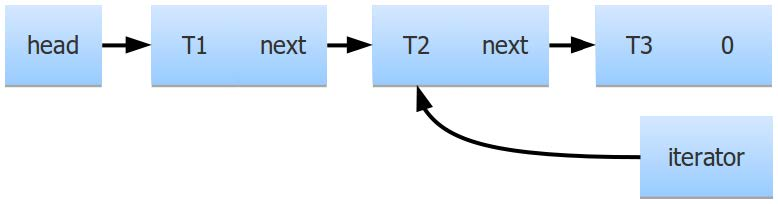
\includegraphics[width=0.9\textwidth]{content/2/chapter7/images/24.jpg}\\
圖7.24 - 帶有迭代器的單鏈表
\end{center}

因為每個元素都單獨分配,所以也可以單獨回收。輕量級分配器用於這些數據結構,其中內存在大塊中分配,這些大塊劃分為節點大小的片段。當一個節點釋放時,內存不會返回給操作系統,而是放在一個空閒列表中,以便應對下一次分配內存的請求。就我們的目的而言,內存直接從操作系統分配,還由專門的分配器處理,與我們的關係不大(後者通常更高效)。

併發程序中,鏈表的迭代器是一個挑戰。如圖7.24,這些迭代器可以指向鏈表中的任何位置。如果有元素從鏈表中刪除,則希望它的內存能夠用於構造和插入另一個元素(如果不這樣做,並保持所有內存直到整個鏈表刪除,重複增加和刪除元素會浪費大量的內存)。但若有指向鏈表節點的迭代器,則不能刪除該節點。在單線程程序中也是如此,但是在併發程序中的管理通常要困難得多。對於可能使用多線程的迭代器,不能通過操作的執行流保證沒有迭代器指向要刪除的元素。本例中,需要迭代器來擴展所指向的鏈表節點的生命週期。當然,這是使用引用計數智能指針的工作,比如\texttt{std::shared\_ptr}。現在,假設鏈表中的所有指針,包括連接節點和迭代器中的指針,都是智能指針(\texttt{std::shared\_ptr}或類似的具有強線程安全保證的指針)。

就像處理順序數據結構一樣,對線程安全的數據結構的第一次嘗試應該是使用鎖保護實現。在確定需要之前,永遠不要設計無鎖數據結構。開發無鎖代碼可能很酷,但找到Bug會很困難。

這裡也需要重新設計部分接口,所有的操作都是事務性的。無論鏈表是否為空,\texttt{pop\_front()}都應該工作。然後,可以用鎖保護所有操作。對於\texttt{push\_front()}和\texttt{pop\_front()}這樣的操作,很可能類似於堆棧或隊列的性能。這份清單還列出了此前沒有面對過的挑戰。

首先,該鏈表支持任意位置插入。對於\texttt{std::forward\_list},在迭代器指向的元素之後插入一個新元素可以使用\texttt{inser\_after()}。若同時在兩個線程上插入兩個元素,希望插入操作可以併發進行,除非這兩個位置非常接近,並且影響相同的節點,但不能用一個鎖來保護整個鏈表。

如果考慮長時間運行的操作,比如在鏈表中搜索具有所需值(或滿足其他條件)的元素,情況會更糟。整個搜索操作中,必須鎖定列表,因此在遍歷列表時不能向列表添加或刪除元素。若經常進行搜索,鏈表是不合適的數據結構,但樹和其他節點數據結構也有相同的問題。若需要遍歷數據結構的大部分,需要在整個操作期間持有鎖,從而阻塞所有其他線程訪問,甚至與當前操作無關的節點上的操作也會阻塞。

當然,如果從未遇到過這些問題,那麼就不必擔心這些問題。若鏈表僅從前後端訪問,那麼用一個鎖保護的列表可能就夠了。在設計併發數據結構時,不必要的通用性令人頭痛。不過這裡,只需要構建需要的內容即可。

大多數時候,節點數據結構並不僅僅是從端點訪問的,或者在樹或圖的情況下,實際上沒有任何端點。如果程序將大部分時間用於操作整個數據結構,那麼鎖定整個數據結構以便一次只有一個線程訪問的方式就無法接受。可以考慮的下一個方法是,分別鎖定每個節點。使用鏈表的情況下,可以向每個節點添加自旋鎖,並在需要更改節點時鎖定該節點。但這種方法遇到了所有基於鎖的解決方案的死敵:死鎖。任何需要操作多個節點的線程都必須獲得多個鎖。假設線程A持有節點1上的鎖,現在需要在節點2之後插入一個新節點,所以它也試圖獲得這個鎖。與此同時,線程B持有節點2上的鎖,它希望在節點1之後刪除節點,因此它試圖獲得該鎖,所以現在兩個線程會處於永遠等待的狀態。這個問題不可避免,因為有太多可以以任意順序獲取的鎖,除非對線程訪問鏈表的方式實施非常嚴格的限制(只持有一個鎖),然後就會面臨活鎖的風險,因為線程會不斷地釋放和重新獲取鎖。

如果需要一個鏈表或另一個節點數據結構來併發訪問,就必須想出一個無鎖的實現。無鎖實現並不容易,更難以寫正確。更好的選擇是提出不需要線程安全節點數據結構的算法,這可以通過將全局數據結構的一部分複製到一個線程特定的結構中,然後由單個線程訪問。在計算結束時,來自所有線程的部分再次放在一起。有時,劃分數據結構更容易,這樣就不會併發訪問節點(例如,可以在一個線程上劃分圖並處理每個子圖,然後處理邊界節點)。但若需要線程安全的節點數據結構該怎麼辦?下一節將解釋其中的挑戰,並提供一些實現選項。

\subsubsubsection{7.5.1\hspace{0.2cm}無鎖鏈表}

無鎖鏈表或其他節點容器的基本思想非常簡單,基於使用比較-交換操作指向節點的指針。讓從更簡單的操作開始:插入。將描述在鏈表頭部進行插入操作,在其他節點之後的插入操作也是一樣的。

%\hspace*{\fill} \\ %插入空行
\begin{center}
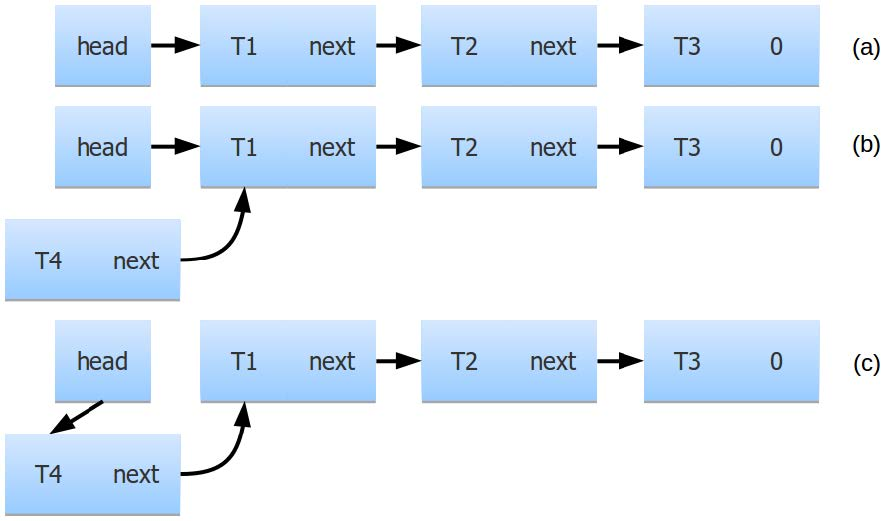
\includegraphics[width=0.9\textwidth]{content/2/chapter7/images/25.jpg}\\
圖7.25 - 在單鏈表頭部插入一個新節點
\end{center}

假設在圖7.25a所示的鏈表頭部插入一個新節點。第一步是讀取當前頭指針,即指向第一個節點的指針。然後用期望值創建新的節點,它的next指針與當前的頭指針相同,所以這個節點在當前第一個節點之前鏈接到鏈表中(圖7.25b)。此時,新節點還不能被其他線程訪問,因此可以併發地訪問數據結構,最後執行CAS。如果當前頭指針沒有改變,將用指向新節點的指針替換它(圖7.25c)。如果頭指針不再具有第一次讀取時的值,則讀取新值,將其寫入新節點的下一個指針,並再次嘗試原子CAS。

這是一個簡單可靠的算法。這是在前一章中看到的發佈協議的應用,新數據是在單線程上創建的,所以不用考慮線程安全(其他線程還不能訪問它)。作為最後的操作,線程通過原子性地更改可訪問所有數據的根指針(我們的例子中是鏈表頭)來發布數據。如果將新節點插入到另一個節點之後,將自動地更改該節點的next指針。唯一的區別是,多個線程可能試圖在同一時間發佈新的數據。為了避免數據競爭,必須使用\textit{比較和交換}。 

現在,考慮相反的操作,擦除鏈表的前端節點。這也是通過三個步驟完成的:

%\hspace*{\fill} \\ %插入空行
\begin{center}
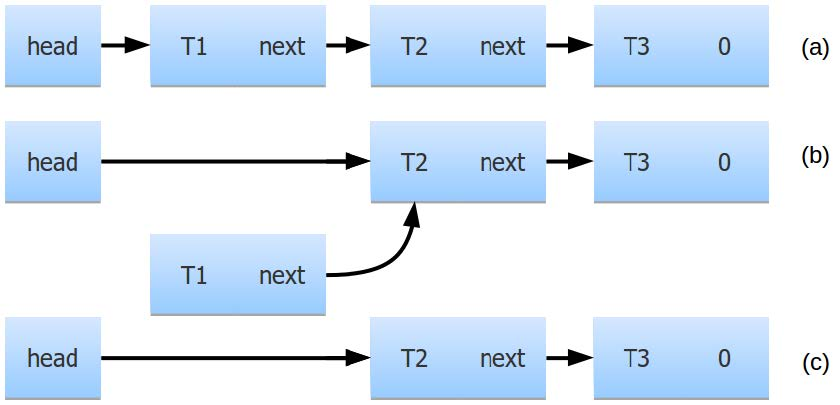
\includegraphics[width=0.9\textwidth]{content/2/chapter7/images/26.jpg}\\
圖7.26 - 單鏈表頭部的無鎖移除
\end{center}

讀取頭指針,使用它訪問鏈表的第一個節點,然後讀取它的next指針(圖7.26a)。然後,將next指針的值原子地寫入頭指針中(圖7.26b),但前提是頭指針沒有改變(CAS)。此時,其他線程訪問不能訪問前面的節點,這樣線程就擁有頭指針的原始值,並且可以使用它來刪除需要刪除的節點(圖7.26c)。但是,當試圖將這兩種操作結合起來時,問題就出現了。

假設兩個線程同時對鏈表進行操作,線程A試圖刪除鏈表中的第一個節點。第一步是讀取頭指針和指向next節點的指針,這個指針即將成為鏈表的新頭,但是比較和交換還沒有發生。現在,這個頭節點是不變的,新頭節點是(head'),它只存在於線程A的某個局部變量中。這個時刻如圖7.27a所示:

%\hspace*{\fill} \\ %插入空行
\begin{center}
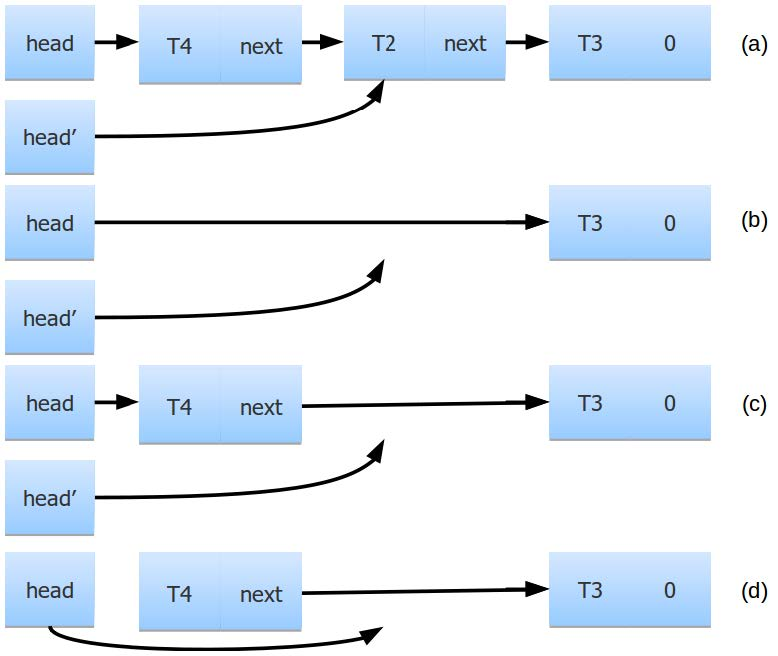
\includegraphics[width=0.9\textwidth]{content/2/chapter7/images/27.jpg}\\
圖7.27 - 單鏈表頭部的無鎖插入和移除
\end{center}

這時,線程B成功地刪除了鏈表的第一個節點。然後它還會刪除下一個節點,使鏈表保持圖7.27b所示的狀態(線程A沒有取得任何進展)。然後,線程B在鏈表的開頭插入一個新節點(圖7.27c)。然而,由於兩個已刪除節點的內存釋放,因此節點T4的新分配重用了之前分配的內存,因此節點T4與原始節點T1擁有了相同的地址。只要刪除節點的內存可用於新的分配,這種情況就大概率會發生。事實上,大多數內存分配器更偏愛返回最近釋放的內存,前提是它還在CPU的緩存中。

現在,線程A終於再次運行了,要做的操作是比較和交換。如果頭指針自線程A上次讀取它後沒有改變,那麼新頭成為了現在的頭(head')。但就線程A所見,頭指針的值仍然是相同的(它法觀察整個更改歷史記錄)。CAS操作成功,新的頭指針現在指向節點T2以前所使用的內存,而節點T4不再可訪問(圖7.27d)。自此,整個鏈表壞了。

這種故障在無鎖數據結構中非常常見,以至於擁有了一個術語:\textbf{A-B-A問題}。 這裡的\textbf{A}和\textbf{B}指的是內存位置,問題是數據結構中的某個指針將其值從A更改為B,然後再返回A。另一個線程只觀察初始值和最終值,根本看不到任何更改。比較和交換操作成功,開發者假定數據結構不變。但這個假設是不正確的,數據結構可以進行改變,但沒觀察到的指針的值的修改,其值就恢復到原來的狀態。

問題的根源在於,如果內存回收和分配,那麼內存中的指針或地址不能作為數據的唯一標識。這個問題有多種解決方案,都通過不同的方式完成了相同的事情。必須確保在讀取了一個將會比較-交換使用的指針時,在比較-交換完成之前(成功或不成功),該地址的內存不能釋放。如果內存沒有釋放,那麼在同一個地址上就不會發生另一次內存分配,這樣就不會出現A-B-A問題。注意,釋放內存與刪除節點是不一樣的。當然,可以使節點不可訪問的數據結構的其餘部分(刪除節點),甚至可以為存儲在節點中的數據使用析構函數,但不釋放節點所佔用的內存。

通過延遲內存回收,出現了許多方法可以用來解決A-B-A問題。若知道算法在數據結構的生命週期內不會刪除很多節點,那麼可以將所有刪除的節點存放在一個延遲釋放的列表中,以便在刪除整個數據結構時刪除它們。這種方法更通用的版本可以描述為垃圾收集,所有釋放的內存先放到一個垃圾收集列表中。垃圾內存週期性地返回給主內存分配器,但是在垃圾收集期間,數據結構上的所有操作都會掛起。正在進行的操作必須在收集開始之前完成,所有新的操作都會阻塞,直到收集完成。這確保了沒有比較和交換操作,也可以跨越垃圾收集的間隔。因此,操作都不會回收內存。現在流行的RCU(read-copy-update)技術也是這種方法的一種變體。另一種常見的方法是使用風險指針。

本書中,將介紹另一種使用原子共享指針的方法(\texttt{std::shared\_ptr}本身不是原子的,但該標準包含了對共享指針進行原子操作所需的必要函數,或者可以為應用程序編寫自定義函數,使其更快)。重新看一下圖7.27b,現在所有的指針都是原子共享指針。只要有一個這樣的指針指向一個節點,該節點就不能釋放。在相同的事件序列中,線程A仍然擁有指向原始節點T1的舊頭指針,以及指向節點T2的新頭指針head'。

%\hspace*{\fill} \\ %插入空行
\begin{center}
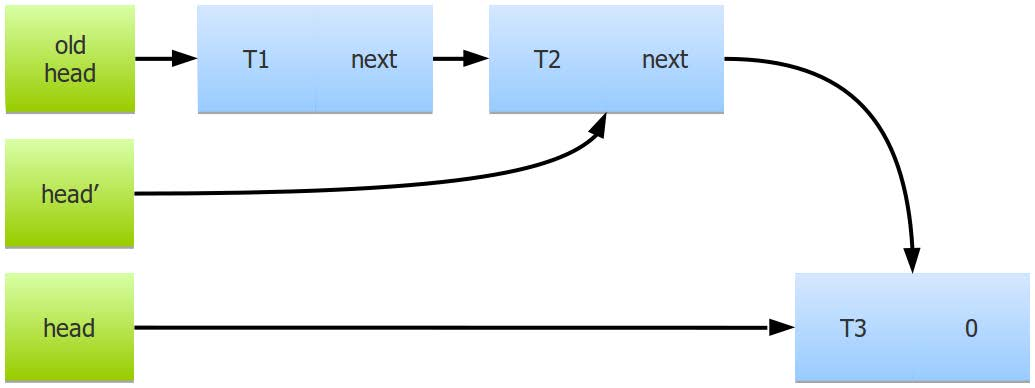
\includegraphics[width=0.9\textwidth]{content/2/chapter7/images/28.jpg}\\
圖7.28 - 使用共享指針的單鏈表頭指針——無鎖插入和移除
\end{center}

線程B已經從鏈表中刪除了兩個節點(圖7.28),但是內存還沒有釋放。不同於當前分配的所有節點的地址,新的節點T4在其他地址上分配。因此,當線程A繼續執行時,會發現新鏈表頭指針與舊頭指針的指向的值不同。比較-交換將失敗,線程A將再次嘗試操作。此時,將重新讀取頭指針(並獲取節點T3的地址)。因為它是指向節點T1的最後一個共享指針,所以頭指針的舊值現在沒有了,這個節點因為沒有更多的引用而刪除了。類似地,只要共享指針head'重置為新的預期值(節點T3的下一個指針),節點T2就會刪除。節點T1和T2都沒有指向它們的共享指針,因此它們最終也會刪除。

當然,這是在節點前插入的情況。為了允許在任何地方插入和刪除,必須將所有指向節點的指針轉換為共享指針。這包括所有節點的next指針,以及指向鏈表迭代器中隱藏的節點的指針。這樣的設計還有另一個優點:解決了鏈表遍歷(如搜索操作)與插入和刪除同時發生的問題。

如果在有指向該鏈表的迭代器時刪除了一個節點(圖7.29),該節點仍然是已分配的,迭代器有效。即使刪除了下一個節點(T3),也不會釋放,因為有一個共享指針指向它(節點T2的下一個指針)。迭代器可以遍歷整個鏈表。

%\hspace*{\fill} \\ %插入空行
\begin{center}
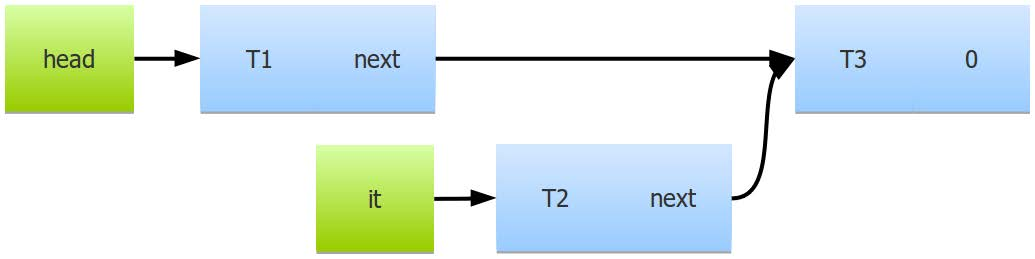
\includegraphics[width=0.9\textwidth]{content/2/chapter7/images/29.jpg}\\
圖7.29 - 使用原子共享指針的無鎖鏈表——線程安全的遍歷
\end{center}

當然,這個遍歷可能包括不再在鏈表中的節點,不需要再從鏈表的頭指針可達的節點開始了。併發數據結構的本質,討論當前內容沒有任何意義。瞭解鏈表內容的唯一方法是從鏈表頭遍歷到最後一個節點,但當迭代器到達鏈表末尾時,之前的節點可能已經改變,遍歷的結果不再是之前那個“鏈表”的結果。這種思維方式需要一些時間來適應。

這裡不打算展示無鎖鏈表與鎖保護鏈表的基準測試,因為這些基準測試必須基於特定的應用程序。如果只對鏈表頭節點的插入和刪除進行基準測試(\texttt{push\_front()}和\texttt{pop\_front()}),那麼由自旋鎖保護的鏈表將會更快(原子共享指針並不便宜)。另一方面,如果對同步插入和搜索進行基準測試,則可以使無鎖鏈表的速度最快。遍歷包含1M個元素的鏈表時,鎖保護的鏈表一直處於鎖定狀態,而無鎖列表可以在每個線程上同時進行迭代,同時進行插入和刪除操作。無論原子指針有多慢,只要使無鎖鏈表足夠長就會快。這並不是毫無根據的觀察,應用程序可能需要執行一些操作,這些操作需要將鏈表鎖定很長時間,除非能夠以某種方式對鏈表進行分區,以避免死鎖。如果需要這樣做,那麼無鎖鏈表就是最快的。如果只需要迭代幾個元素,並且從不同時在許多不同的位置,那麼用鎖保護鏈表就可以了。

A-B-A問題和解決方案不僅適用於鏈表,也適用於所有節點數據結構:雙鏈表、樹和圖。由多個指針鏈接的數據結構中,可能會遇到其他問題。首先,即使所有指針都是原子指針,一個接一個地更改兩個原子指針也不是一個原子操作。這將導致數據結構中的臨時不一致。期望從一個節點到下一個節點,然後返回到前一個節點,這樣就回到了原始節點。但在併發情況下,這並不總是正確的。如果在這個位置插入或刪除節點,其中一個指針可能會在另一個指針之前更新。第二個問題是特定於共享指針或其他使用引用計數的實現,若數據結構有指針循環,循環中的節點也不會刪除,即使沒有有外部引用。最簡單的例子是雙鏈表,其中兩個相鄰的節點總是有指向彼此的指針。在單線程程序中,解決這個問題的方法是使用弱指針(在雙鏈表中,所有的next指針都可以共享,所有的前一個指針都是弱指針)。這對於併發程序來說不是很好,關鍵是延遲內存回收,直到沒有更多的引用才進行,而弱指針不會這樣做。對於這些情況,可能需要額外的垃圾收集機制。在最後一個指向節點的外部指針刪除後,必須遍歷鏈接的節點,並檢查是否有外部指針指向它們(可以通過檢查引用計數來做到),沒有外部指針的鏈表可以安全刪除。對於這類數據結構,可以使用風險指針或顯式垃圾收集等替代方法。讀者可以參閱有關無鎖編程的書籍,以獲得關於這些方法的更多信息。

好了,現在可以結束對並行編程高性能數據結構的探索了。現在來總結一下了解到的知識。













